\documentclass{article}
\usepackage[height=25cm, a4paper, hmargin={3cm, 2cm}]{geometry}
\usepackage[T1,T2A]{fontenc}
\usepackage[utf8]{inputenc}
\usepackage[english,russian]{babel}
\usepackage[section]{placeins}
\usepackage{graphicx}
\usepackage{lscape}
\usepackage{pdflscape}
\usepackage{minted}
\usepackage{amsmath}
\usepackage{wrapfig}
\usepackage[numbered, framed]{matlab-prettifier}
\graphicspath{{}}

\makeatletter
\long\def\@makecaption#1#2{%
  \vskip\abovecaptionskip
  \hbox to\textwidth{\hfill\parbox{0.8\textwidth}{\begin{center}#1: #2\end{center}}\hfill}
  \vskip\belowcaptionskip}
\makeatother

\begin{document}
	\pagestyle{empty}
	\begin{titlepage}
	\begin{center}
        \large{
            Министерство образования и науки Российской Федерации\\Федеральное государственное автономное образовательное учреждение высшего образования}\\
        \vspace*{3em plus 7em minus 6em}
        \Large
        САНКТ-ПЕТЕРБУРГСКИЙ НАЦИОНАЛЬНЫЙ ИССЛЕДОВАТЕЛЬСКИЙ \\УНИВЕРСИТЕТ ИНФОРМАЦИОННЫХ ТЕХНОЛОГИЙ, МЕХАНИКИ И ОПТИКИ\\
        \vspace*{3em plus 7em minus 6em}
        \Large
        Факультет систем управления и робототехники\\
        \vspace*{7em plus 7em minus 6em}
        \LARGE
        {\bf
        Отчет по лабораторной работе №7 \\ <<Прямая и обратная задача кинематики. DH-параметры>> \\по дисциплине <<Введение в профессиональную деятельность>>}\\
    \end{center}
	\begin{flushright}
		\Large
		\vspace*{10em plus 11em minus 9em}
		Выполнили студенты гр. {\textbf {R3135}}\\
		Трубицына А.М.\\
		Вьюгина А.П.\\
		Репин А.В.\\
		Макаренко К.С.\\
		Преподаватель: Перегудин А.А.,\\
		ассистент фак. СУиР		
	\end{flushright}
	\vspace*{15em plus 7em minus 6em}
	\begin{center}
		Санкт-Петербург 2020
	\end{center}
	\end{titlepage}


\section{Цель работы}
Ознакомиться со способом нахождения параметров манипулятора и научиться переходить из декартовых координат в обобщенные и обратно.

\section{Описание собранного робота}
\subsection*{Фотографии собранного робота}
\begin{figure}[h!]
    \begin{minipage}{.55\textwidth}
        \centering
        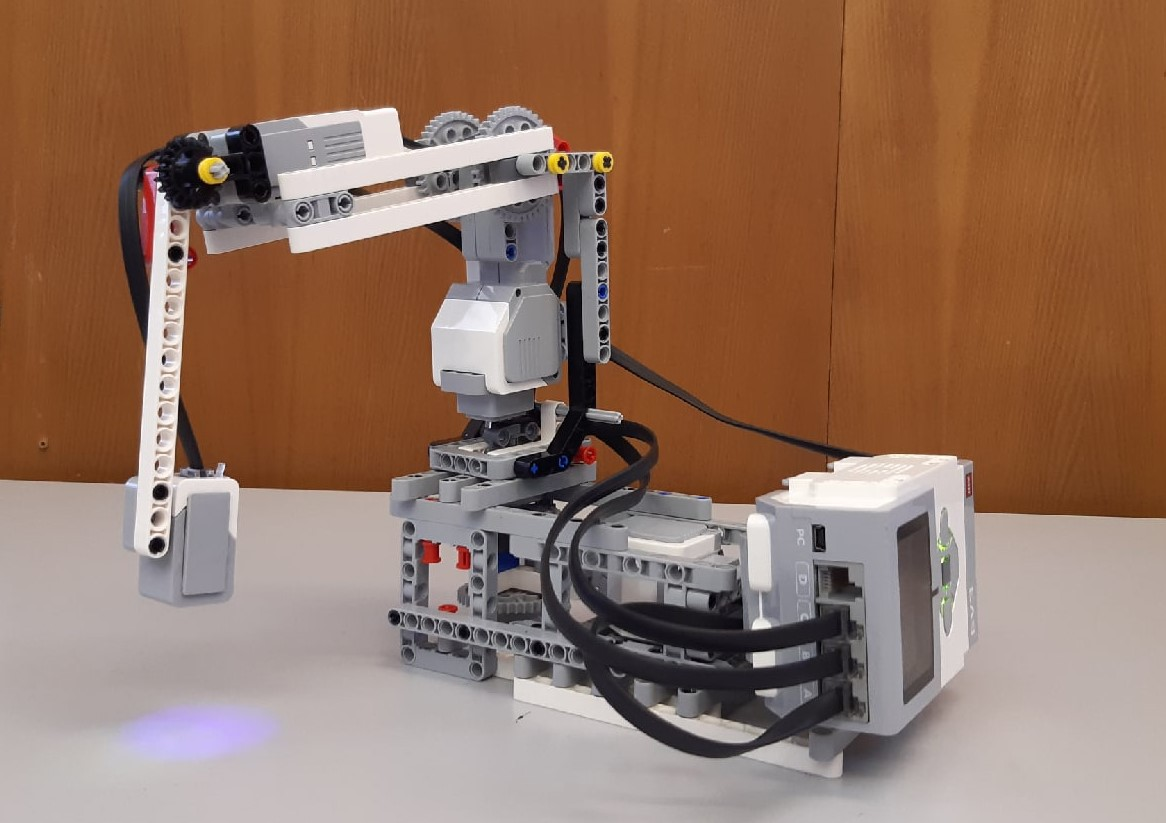
\includegraphics[width=250 pt]{robot_photo1.jpg}
    \end{minipage}
    \begin{minipage}{.55\textwidth}
        \centering
        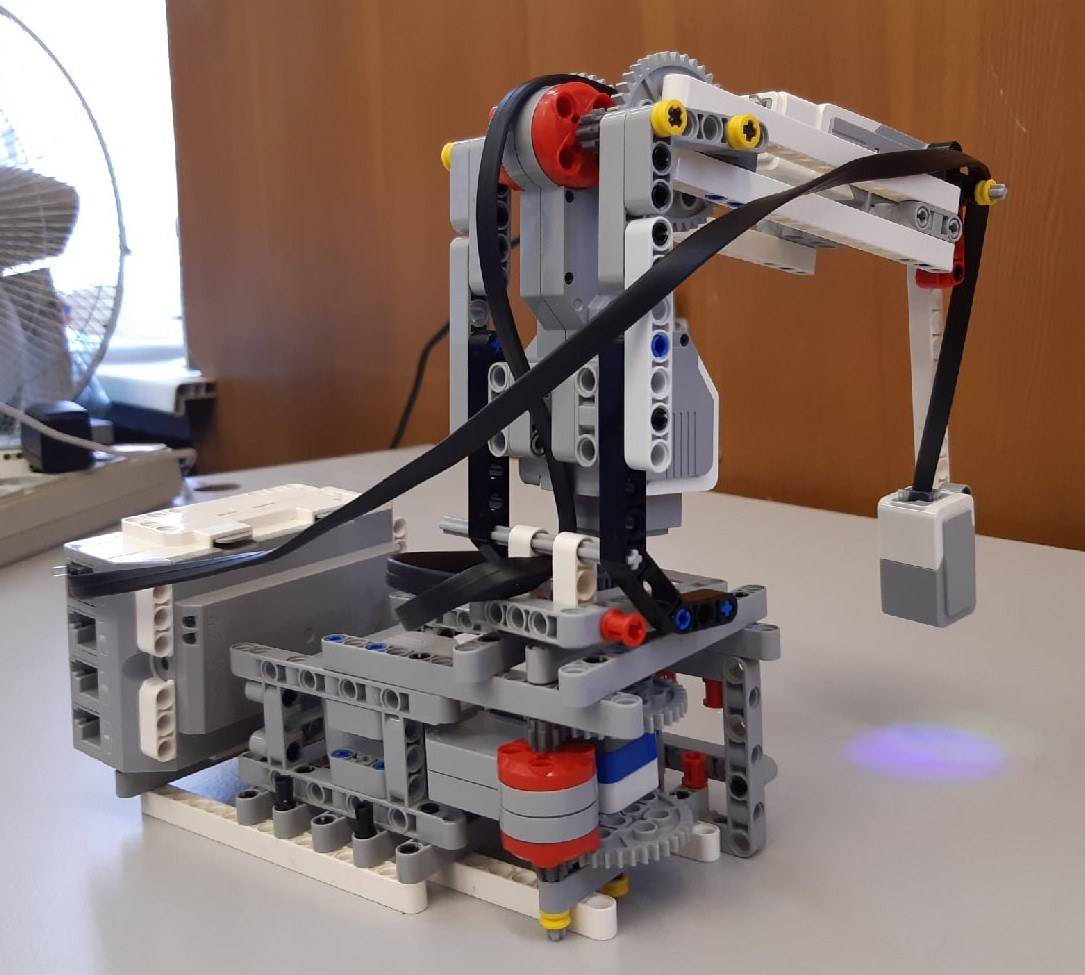
\includegraphics[width=198 pt]{robot_photo2.jpg}
    \end{minipage}
    \caption{Фотографии робота}
\end{figure}
\FloatBarrier
\par У первого и второго мотора передаточное отношение равно 5, у третьего - $\frac{5}{3}$ (при нумерации моторов снизу вверх).
\subsection*{Параметры Денавита-Харденберга}
\par Для упрощения расчетов и использования четырех величин вместо 6 можно использовать параметры Денавита-Хартенберга. Это один из наиболее общих способов определить координаты хвата манипулятора по обобщенным координатам манипулятора (т. е. по углам, на которые поворачиваются звенья). Безусловно, координаты можно рассчитать и геометрически, как сделано далее, но в случае, когда звеньев много, этот способ оказывается неудобным. \\

\begin{tabular}{|l||c|c|c|c|}
\hline
Звено i & $a_i$ & $\alpha_i$ & $d_i$ & $\theta_i$\\
\hline
\hline
1 & 0,7 см & $\frac{\pi}2$ & 18 см & $\theta_1$  \\ \hline
2 & 12,8 см & 0 & 0 & $\theta_2$ + $\frac{\pi}2$ \\ \hline
3 & 12,8 см & 0 & 0 & $\theta_3$\\
\hline
\end{tabular}

\section{Коды для перехода из одной системы координат в другую}
\subsection{Функция для перехода из обобщенной СК в Декартову с помощью геометрических расчетов}
\subsubsection*{Вывод формул}
\begin{figure}[h!]
\begin{minipage}{.65\textwidth}
\centering
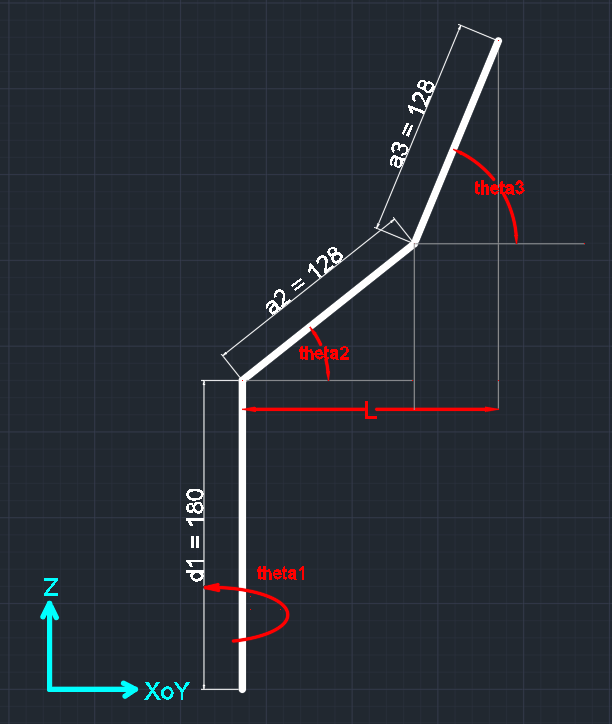
\includegraphics[width=200 pt]{str_formulas.png}
\caption{Чертеж для вывода указанных формул}
\end{minipage}
\begin{minipage}{.35\textwidth}
\centering
Из чертежа: 
\begin{equation*}
    \begin{cases}
        z = d_1 + a_2\sin{\theta_2} + a_3\sin{\theta_3} \\
        L = a_2\cos{\theta_2} + a_3\cos{\theta_3}
    \end{cases}
\end{equation*}

Тогда итоговый результат равен\\
\begin{equation*}
    \begin{cases}
        x = \cos{\theta_1}(a_2\cos{\theta_2} + a_3\cos{\theta_3}) \\
        y = \sin{\theta_1}(a_2\cos{\theta_2} + a_3\cos{\theta_3}) \\
        z = d_1 + a_2\sin{\theta_2} + a_3\sin{\theta_3}
    \end{cases}
\end{equation*}

\end{minipage}
\end{figure}
\FloatBarrier

\subsubsection*{Код}
\begin{minted}[linenos=true]{python}
def straight_transfer_formulas(theta1, theta2, theta3):
    theta3 = theta2-theta3
    theta1 = np.deg2rad(theta1)
    theta2 = np.deg2rad(theta2)
    theta3 = np.deg2rad(theta3)
    a = [0, 0.007, 0.128, 0.128]  # массив значений a_i
    alpha = [0, pi / 2, 0, 0]
    d = [0, 0.18, 0, 0]  # массив значений d_i
    x = (a[2] * cos(theta2) + a[3] * cos(theta3)) * cos(theta1)
    y = (a[2] * cos(theta2) + a[3] * cos(theta3)) * sin(theta1)
    z = d[1] + a[2] * sin(theta2) + a[3] * sin(theta3)
    print("x = ", x)
    print("y = ", y)
    print("z = ", z)

\end{minted}


\subsection{Функция для перехода из обощенной СК в Декартову с помощью матричных расчетов}

\subsubsection*{Вывод формул}
Матрица перехода из обобщенной СК в Декартову является произведением матриц перехода от $i-1$-го звена к $i$-ому: $T^0_n=T^0_1 \cdot T^1_2 \cdot T^2_3 $. \\
Итоговая матрица - результат следующего выражения:
\begin{center}
$T^0_3 = \begin{bmatrix}
\cos{\theta_1} & -\sin{\theta_1} \cos{\alpha_1} & \sin{\theta_1} \sin{\alpha_1} & a_1 \cos{\theta_1} \\
\sin{\theta_1} & \cos{\theta_1} \cos{\alpha_1} & -\cos{\theta_1} \sin{\alpha_1} & a_1 \sin{\theta_1} \\
0 & \sin{\alpha_1} & \cos{\alpha_1} & d_1\\
0 & 0 & 0 & 1\\
\end{bmatrix}
\cdot
\begin{bmatrix}
\cos{\theta_2} & -\sin{\theta_2} \cos{\alpha_2} & \sin{\theta_2} \sin{\alpha_2} & a_2 \cos{\theta_2} \\
\sin{\theta_2} & \cos{\theta_2} \cos{\alpha_2} & -\cos{\theta_2} \sin{\alpha_2} & a_2 \sin{\theta_2} \\
0 & \sin{\alpha_2} & \cos{\alpha_2} & d_2\\
0 & 0 & 0 & 1\\
\end{bmatrix}
\cdot
\begin{bmatrix}
\cos{\theta_3} & -\sin{\theta_3} \cos{\alpha_3} & \sin{\theta_3} \sin{\alpha_3} & a_3 \cos{\theta_3} \\
\sin{\theta_3} & \cos{\theta_3} \cos{\alpha_3} & -\cos{\theta_3} \sin{\alpha_3} & a_3 \sin{\theta_3} \\
0 & \sin{\alpha_3} & \cos{\alpha_3} & d_3\\
0 & 0 & 0 & 1\\
\end{bmatrix}$
\end{center}

\subsubsection*{Код}
\begin{minted}[linenos=true, breaklines=true]{python}
def straight_transfer(theta1, theta2, theta3):
    theta3 = -theta3
    # перевод из градусов в радианы
    theta1 = np.deg2rad(theta1)
    theta2 = np.deg2rad(theta2)
    theta3 = np.deg2rad(theta3)
    Q = np.array([[0], [0], [0], [1]])

    a = [0, 0, 0.128, 0.128]  # массив значений a_i
    alpha = [0, pi / 2, 0, 0]
    d = [0, 0.18, 0, 0]  # массив значений d_i

    T_0_1 = np.array([[cos(theta1), -sin(theta1) * cos(alpha[1]), sin(theta1) * sin(alpha[1]), a[1] * cos(theta1)],
                      [sin(theta1), cos(theta1) * cos(alpha[1]), -cos(theta1) * sin(alpha[1]), a[1] * sin(theta1)],
                      [0, sin(alpha[1]), cos(alpha[1]), d[1]],
                      [0, 0, 0, 1]])

    T_1_2 = np.array([[cos(theta2), -sin(theta2) * cos(alpha[2]), sin(theta2) * sin(alpha[2]), a[2] * cos(theta2)],
                      [sin(theta2), cos(theta2) * cos(alpha[2]), -cos(theta2) * sin(alpha[2]), a[2] * sin(theta2)],
                      [0, sin(alpha[2]), cos(alpha[2]), d[2]],
                      [0, 0, 0, 1]])

    T_2_3 = np.array([[cos(theta3), -sin(theta3) * cos(alpha[3]), sin(theta3) * sin(alpha[3]), a[3] * cos(theta3)],
                      [sin(theta3), cos(theta3) * cos(alpha[3]), -cos(theta3) * sin(alpha[3]), a[3] * sin(theta3)],
                      [0, sin(alpha[3]), cos(alpha[3]), d[3]],
                      [0, 0, 0, 1]])
    T = T_0_1.dot(T_1_2).dot(T_2_3)
    XYZ = T.dot(Q)
    print("x = ", XYZ[0][0])
    print("y = ", XYZ[1][0])
    print("z = ", XYZ[2][0])
\end{minted}

\subsection{Функция для перехода из Декартовой СК в обобщенную}
\begin{minted}[linenos=true]{python}
def backwards_transfer(x, y, z):
    a = [0, 0, 0.128, 0.128]  # массив значений a_i
    d = [0, 0.18, 0, 0]  # массив значений d_i
    r1 = sqrt(x ** 2 + y ** 2)
    r2 = z - d[1]
    r3 = sqrt(r1 ** 2 + r2 ** 2)
    
    theta1 = atan(y / x)
    psi1 = acos((a[2] ** 2 + r3 ** 2 - a[3] ** 2) / (2 * a[2] * r3))
    psi2 = atan(r2 / r1)
    theta2 = psi2 + psi1
    psi3 = acos((a[2] ** 2 + a[3] ** 2 - r3 ** 2) / (2 * a[2] * a[3]))
    theta3 = pi - psi3

    theta1 = np.rad2deg(theta1)
    theta2 = np.rad2deg(theta2)
    theta3 = np.rad2deg(theta3)

    print("theta1 = ", theta1)
    print("theta2 = ", theta2)
    print("theta3 = ", theta3)
\end{minted}

\section{Код для движения робота}
\subsection{Поочередный поворот звеньев манипулятора на заданные углы}
\begin{minted}[linenos=true, breaklines=true]{python}
from ev3dev.ev3 import *
import time


def saturate(x, left, right):
    if x > right: x = right
    if x < left: x = left
    return x


sound = Sound()
sound.set_volume(100)
sound.beep()

# первая координата - motorA
# вторая координата - motorB
# третья координата - motorC
q0 = [90, 45, 45]

# калибровка координат
q0 = [saturate(q0[0], -180, 180), saturate(q0[1], -70, 40), saturate(q0[2], -120, 100)]
q = [5 * q0[0], -5 * q0[1], -5/3 * q0[2]]

# значение коэффициентов в градусных мерах
k_p = [0.3, 0.3, 0.1]
k_i = [0.25/60, 0.25/60, 0]
k_d = [1/60, 1/60, 0]


motorA = LargeMotor('outA')
motorB = LargeMotor('outB')
motorC = MediumMotor('outC')

motorA.position = 0
motorB.position = 0
motorC.position = 0

timeStart = time.time()
last_t = time.time()
sum = 0
last_e = 0
inaccuracy = 5  # погрешность в градусах
U_max = 6.97

name = str(q0[0]) + "_" + str(q0[1]) + "_" + str(q0[2]) + ".txt"
file = open(name, 'w')

motors_set = [motorA, motorB, motorC]

for i in range(3):
    while abs(q[i] - motors_set[i].position) > inaccuracy:
        e = q[i] - motors_set[i].position
        dt = time.time() - last_t
        U = k_p[i] * e + k_d[i] * (e - last_e) / dt + k_i[i] * sum * dt
        U = U/U_max*100
        motors_set[i].run_direct(duty_cycle_sp=saturate(U, -100, 100))
        file.write(str(motorA.position) + '\t' + str(motorB.position) + '\t' + str(motorC.position) + '\t' + str(
            saturate(U, -100, 100)) + '\t' + str(k_p[i] * e) + '\t' + str(k_d[i] * (e - last_e) / dt) + '\t' +
                   str(k_i[i] * sum * dt) + '\n')
        sum += e
        last_e = e
        last_t = time.time()
    sum = 0
    last_e = 0
    last_t = time.time()
    motors_set[i].run_direct(duty_cycle_sp=0)

file.close()
\end{minted}

\par Код, реализующий движение по нескольким заданным точкам, аналогичен вышеуказанному, с единственной разницей в том, что есть массив массивов с точками, которые необходимо обойти, и внешний цикл \mintinline{python}{for j in range(n)}.

\subsection{Одновременный поворот звеньев манипулятора на заданные углы}
\par Единственное отличие от кода, представленного выше, заключается в следующем участке, где определяется управляющее воздействие.
\begin{minted}[linenos=true, breaklines=true]{python}
while abs(q[0] - motors_set[0].position) > inaccuracy or abs(q[1] - motors_set[1].position) > inaccuracy or abs(q[2] - motors_set[2].position) > inaccuracy:
    for i in range(3):
        e[i] = q[i] - motors_set[i].position
        dt = time.time() - last_t
        U[i] = k_p[i] * e[i] + k_d[i] * (e[i] - last_e[i]) / dt + k_i[i] * sum[i] * dt
        U[i] = U[i]/U_max*50
        sum[i] += e[i]
        last_e[i] = e[i]
        last_t = time.time()
        if abs(q[i] - motors_set[i].position) > inaccuracy: motors_set[i].run_direct(duty_cycle_sp=saturate(U[i], -100, 100))
    file.write(str(motorA.position) + '\t' + str(motorB.position) + '\t' + str(motorC.position) + '\n')
\end{minted}



\section{Построенные в Matlab траектории движения робота}
\subsection{Скрипт на Matlab}
\begin{minted}[linenos=true, frame=single,framesep=10pt,breaklines=true, breakafter=true]{Matlab}
results=dlmread('C:\Users\Anastasia\PycharmProjects\Robotics_Lab7\OUT 25.05\square2\square2_4___-90_90_0.txt'); %считываем файл
theta1=results(:,1);
theta2=results(:,2);
theta3=results(:,3);


theta1 = theta1*pi/180/5;
theta2 = theta2*pi/180/(-5);
theta3 = theta3*pi/180/(-5/3);
theta3 = theta2-theta3;

a = [ 0.007, 0.128, 0.128];
d = [ 0.18, 0, 0];
for i = 1:size(results)
    x(i)=(a(2)*cos(theta2(i)) + a(3)*cos(theta3(i)))*(cos(theta1(i)));
    y(i) = (a(2) * cos(theta2(i)) + a(3) * cos(theta3(i)))*(sin(theta1(i)));
    z(i) = d(1) + a(2) * sin(theta2(i)) + a(3) * sin(theta3(i));
end 

hold on; 
line = plot3(x,y,z, 'magenta');
line.LineWidth = 2.5;
grid on;

\end{minted}

\subsection{Построенные графики}
\begin{figure}[h!]
    \centering
    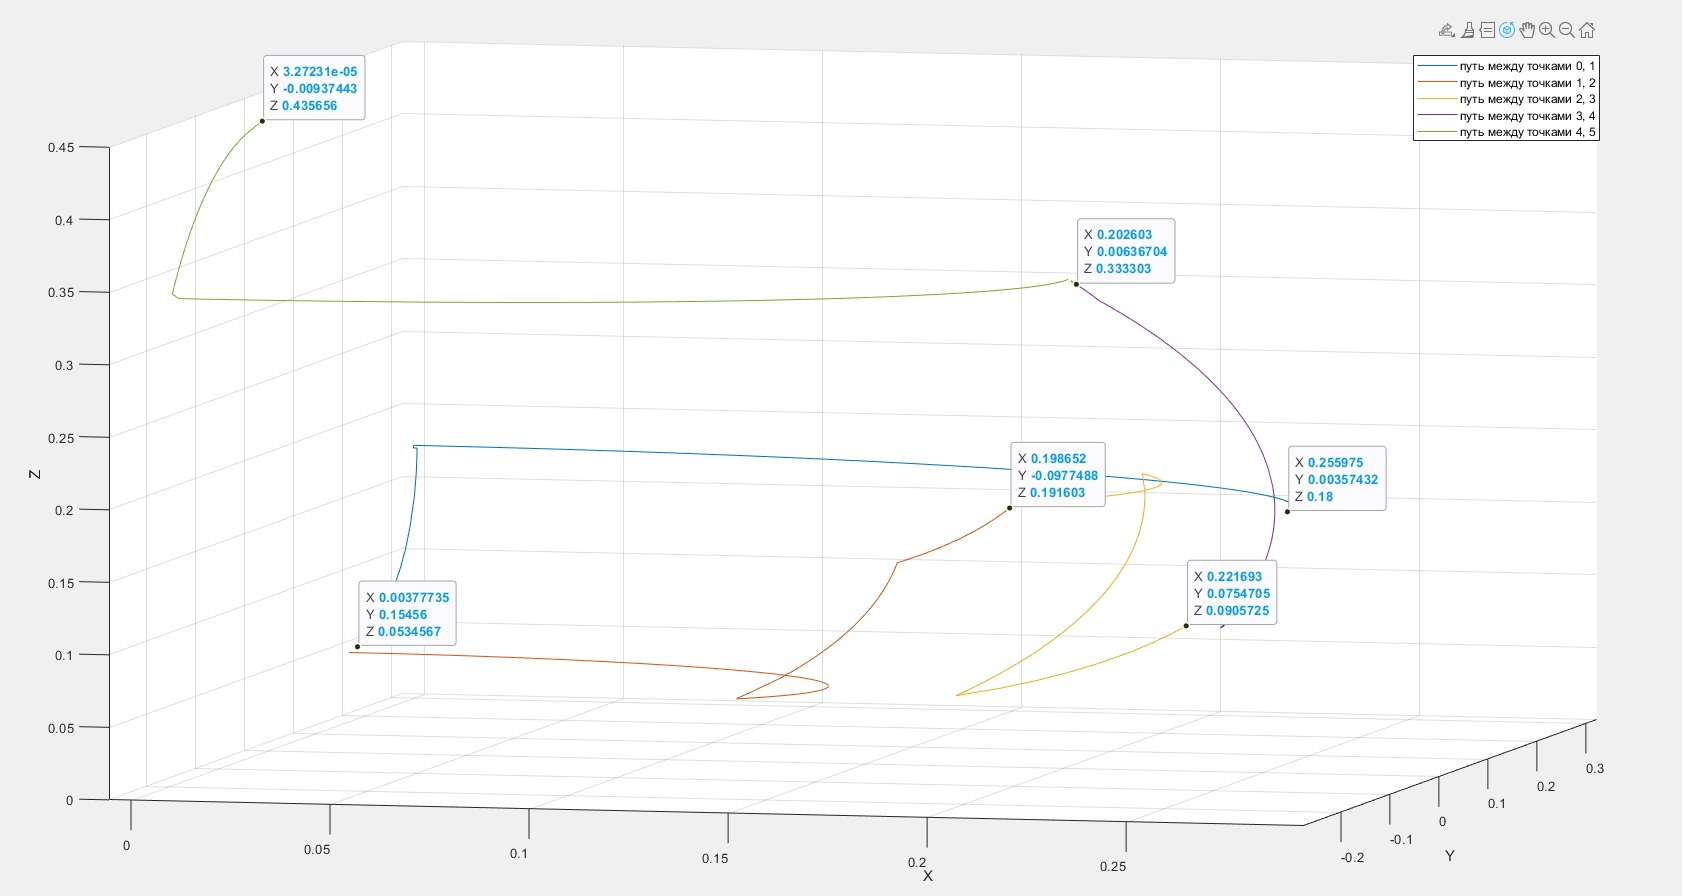
\includegraphics[width=500 pt]{travel_1.jpg}
    \caption{Обход манипулятором 5 точек с поочередным вращением моторов}
\end{figure}
\FloatBarrier
\begin{figure}[h!]
    \centering
    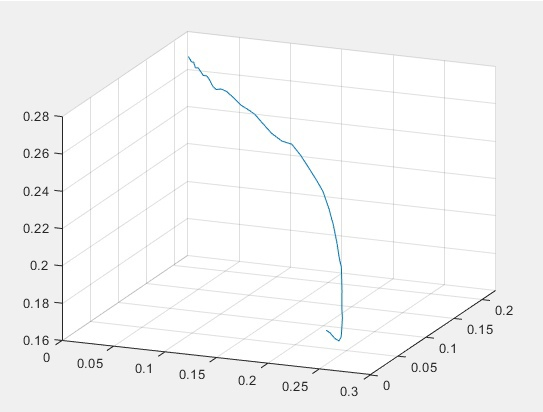
\includegraphics[width=300 pt]{travel_2.jpg}
    \caption{Перемещение в точку с одновременным вращением моторов}
\end{figure}
\FloatBarrier


\section{Использование датчика цвета ColorSensor}
\par В процессе работы появилась идея с помощью манипулятора реализовать механизм, который будет определять цвет предмета и записывать его координату.
\begin{floatingfigure}[l]{3.5 cm}
    \noindent
    \hfill
    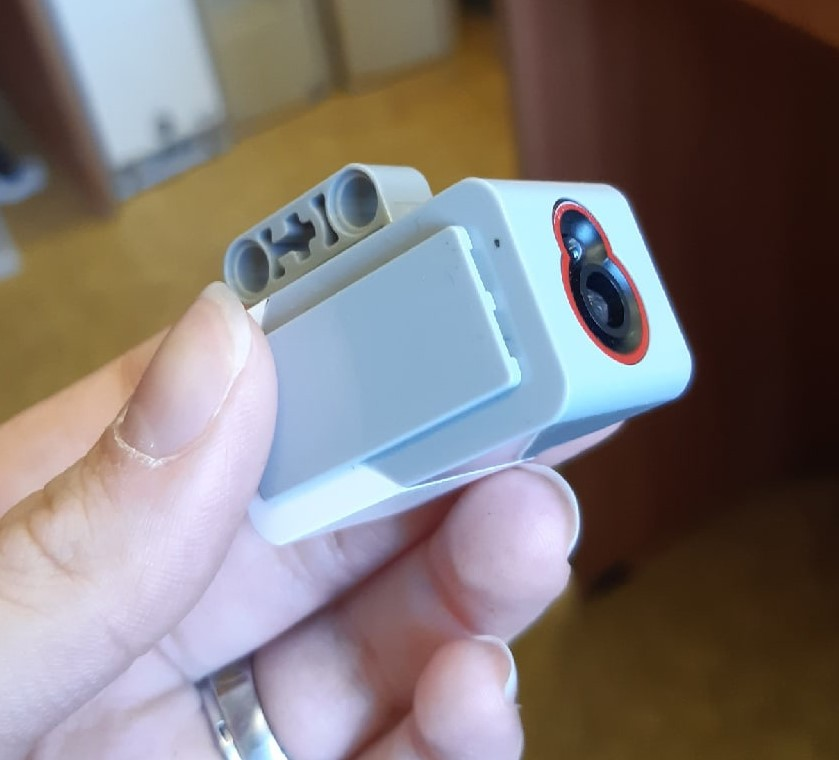
\includegraphics[width=.2\textwidth]{color_sensor.jpg}
    \hfill
\end{floatingfigure}
\par Так как датчик определяет цвета достаточно неточно, то мы придумали некоторый алгоритм калибровки для попадания в классический 8-битный RGB интервал. Для этого мы удерживали датчик, смотрящий на белую бумагу, в одном положении, искали максимальное значение каждой компоненты света. В файл записывалось текущее значение компоненты, деленной на соответствующую максимальную и умноженное на 255. Также возникла идея построить график каждой из компонент и выделить пиковые значения. 


\subsection{Скрипты для реализации этой задачи}
\subsubsection*{Код для калибровки датчика}
\begin{minted}[linenos=true, breaklines=true]{python}
red_component = blue_component = green_component = 0
counter = 0
while time.time() - time_start < 0.5:
    counter += 1
    red_component += color_sensor.value(0)
    green_component += color_sensor.value(1)
    blue_component += color_sensor.value(2)
red_ideal = red_component/counter
green_ideal = green_component/counter
blue_ideal = blue_component/counter
\end{minted}
\subsubsection*{Код для построения графиков}
\begin{minted}[linenos=true, frame=single,framesep=10pt,breaklines=true, breakafter=true]{Matlab}
results=dlmread('C:\Users\Anastasia\PycharmProjects\Robotics_Lab7\OUT 8.06\code_color2.txt'); %считываем файл
time = results(:, 1);
red = results(:, 5);
green = results(:, 6);
blue = results(:, 7);
hold on;
plot(time, red, 'r');
plot(time, green, 'g');
plot(time, blue, 'b');
\end{minted}

\subsection{Полученный график интенсивностей RGB-компонент отраженного света}
\begin{figure}[h]
    \centering
    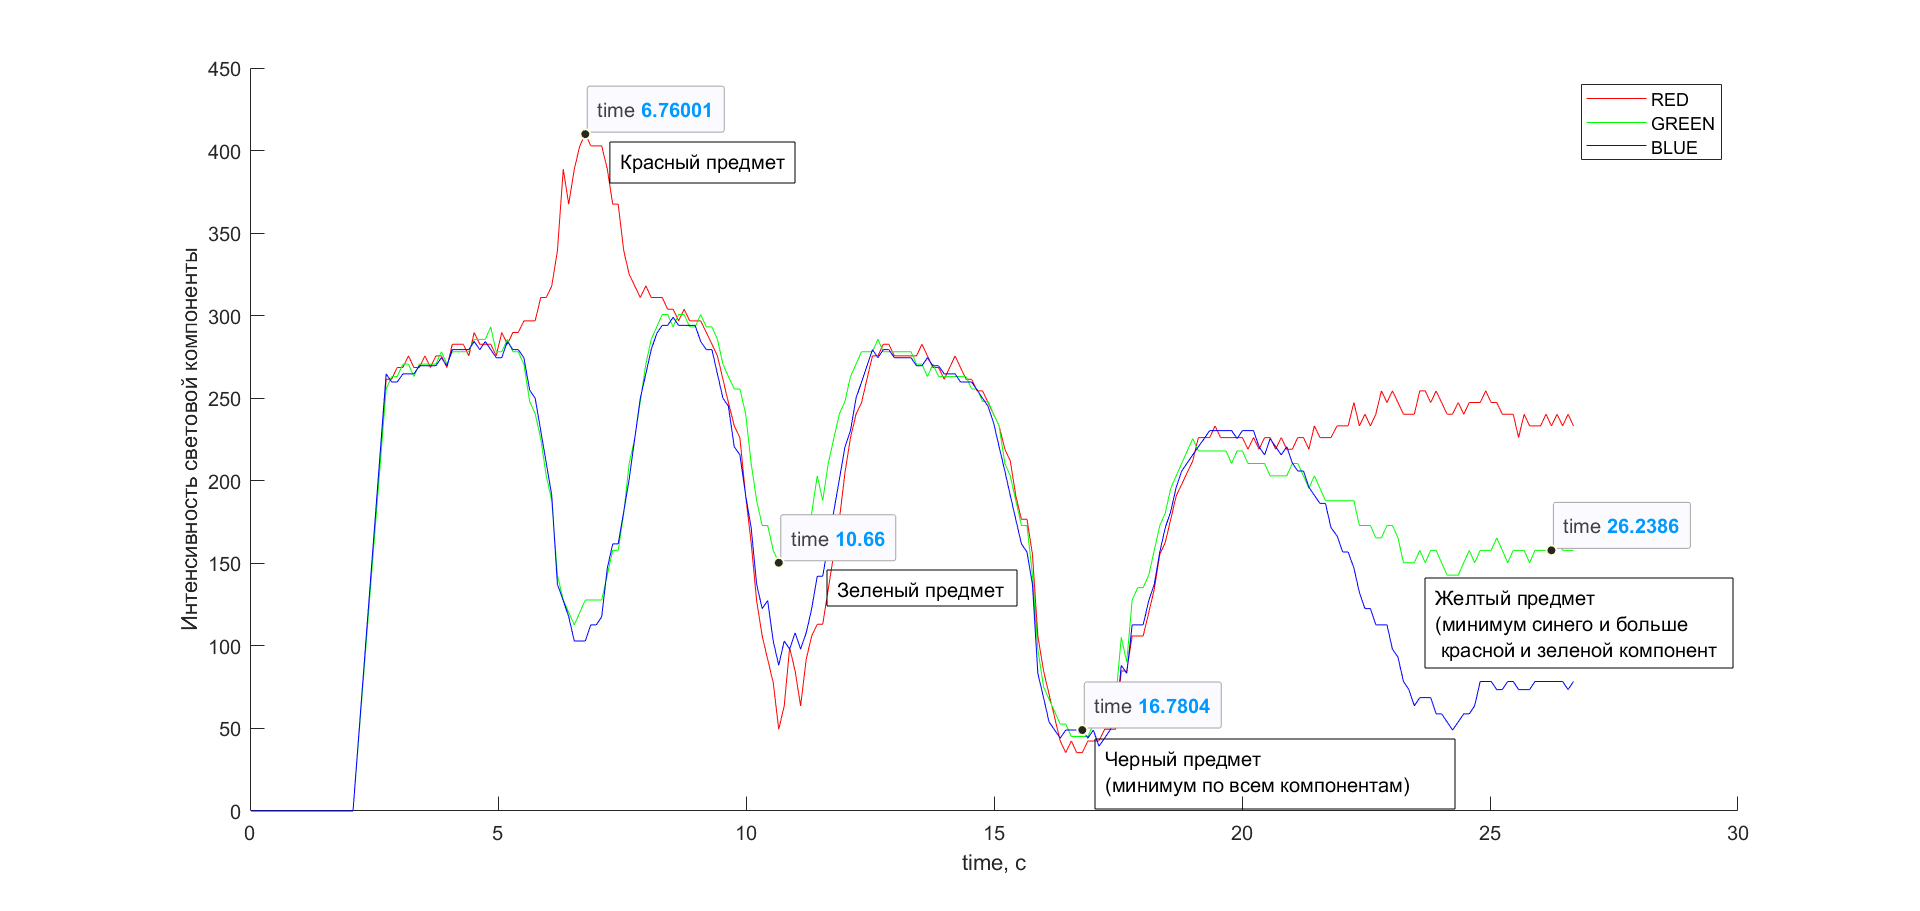
\includegraphics[width=500 pt]{color_graph.png}
    \caption{График интенсивностей компонент}
\end{figure}

\par При анализе графика можно заметить 4 момента времени, в которые так или иначе устанавливается некоторое пиковое(т. е. максимальное или минимальное) значение по какой-то из компонент.
\begin{itemize}
\item Максимальное значение у красного, минимальные у синего и зеленого определяют красный цвет
\item Значение эеленого больше, чем у синего и красного - значит, цвет - зеленый
\item Минимум по всем компонентам определяет черный цвет
\item Смесь красного и зеленого с минимальным количеством синего определяет желтый цвет. На этом моменте манипулятор замер, поэтому это значение является не пиковым, а установившимся. Однако, если бы робот продолжил движение, то значения бы также продолжили меняться.
\end{itemize}

\par Тогда, если проводить расчет для каждой точки, то получаются следующий результаты:
\begin{itemize}
\item Координата красной крышки: $(0.07 , -0.08 , 0)$
\item Координата зеленого объекта: $(0.1 , -0.025 , 0)$
\item Координата черной крышки: $(0.09 , 0.06 , 0)$
\item Координата желтой детали: $(0.02 , 0.11 , 0)$
\end{itemize}
Координата z у всех трех объектов нулевая, потому что они лежат в плоскости $XoY$.
\par Действительно, аналитические выкладки верны, так как на самом деле ситуация выглядела следующим образом:
\begin{figure}[h!]
    \centering
    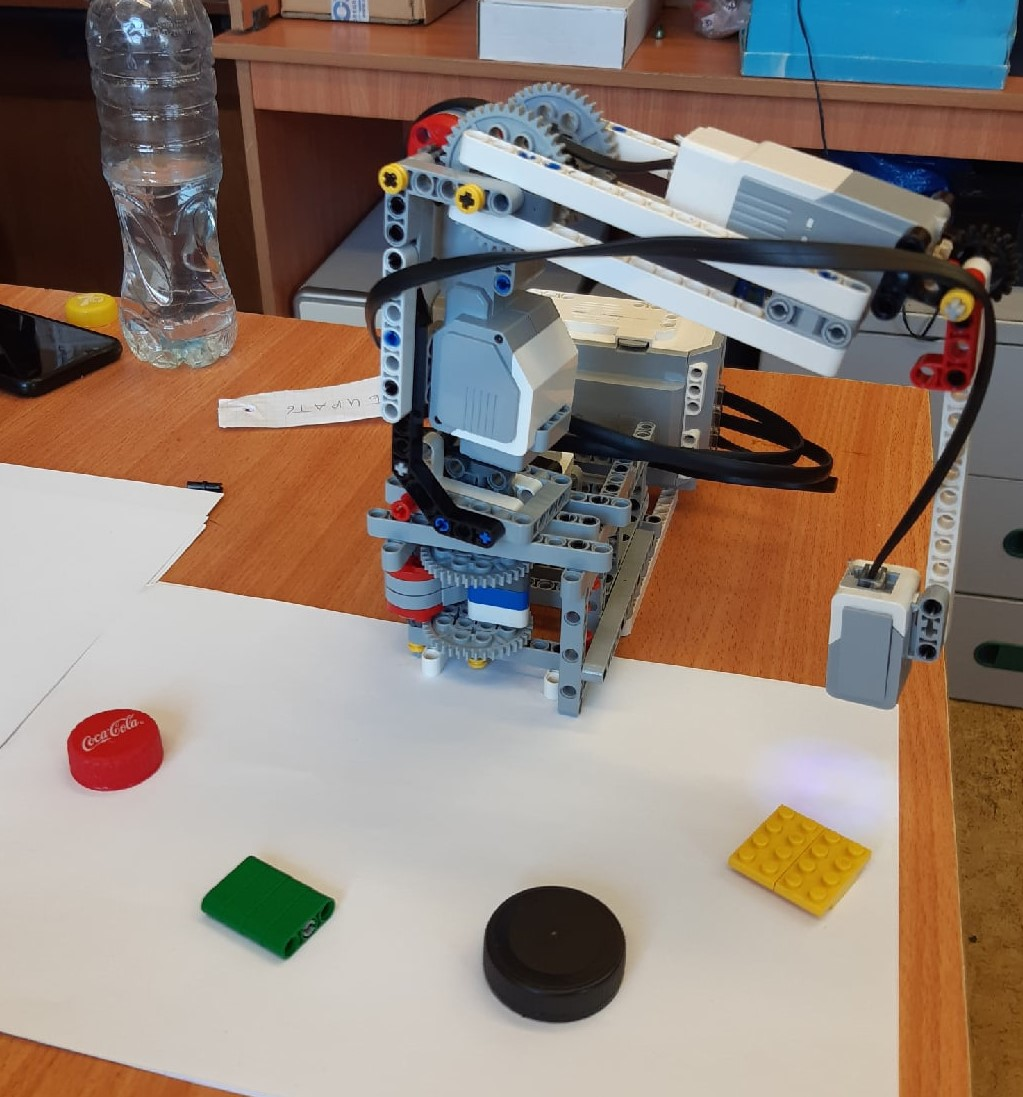
\includegraphics[width=300 pt]{robot_cups.jpg}
    \caption{Робот с крышками}
\end{figure}

\section{Выводы}
\par В процессе выполнения лабораторной работы ознакомились со способами нахождения параметров манипулятора и научились переходить из декартовых координат в обобщенные и обратно.
\par Более того, была поставлена задача - научить робота распознавать цвета и узнать координату предмета того или иного цвета. Задача выполняется в полуавтоматическом режиме - робот записывает данные в файл, затем происходит ручной анализ графика и выборка необходимых углов, по которым в дальнейшем происходит расчет координат.
\end{document}
